\documentclass[11pt, oneside, twocolumn, reqno]{article}   	% use "amsart" instead of "article" for AMSLaTeX format
\usepackage{geometry}                		% See geometry.pdf to learn the layout options. There are lots.
\geometry{letterpaper}                   		% ... or a4paper or a5paper or ... 
%\geometry{landscape}                		% Activate for rotated page geometry
\usepackage[parfill]{parskip}    		% Activate to begin paragraphs with an empty line rather than an indent
\usepackage{graphicx}				% Use pdf, png, jpg, or eps§ with pdflatex; use eps in DVI mode
								% TeX will automatically convert eps --> pdf in pdflatex		
\usepackage{amssymb}

%SetFonts

%SetFonts

\usepackage{gensymb}

\usepackage[cmex10]{amsmath}
\usepackage{amsthm}
\usepackage[export]{adjustbox}
\usepackage{bm}
\usepackage{longtable}
\usepackage{enumitem}
\usepackage{mathtools}
 \usepackage{tikz}
\usepackage[breaklinks=true]{hyperref}
\usepackage{listings}
\usepackage{color}                                            
\usepackage{array}                                            
\usepackage{longtable}                                      
\usepackage{calc}                                             
\usepackage{multirow}                                      
\usepackage{hhline}                                          
\usepackage{ifthen}                                           
\usepackage{lscape}     
\usepackage{multicol}

\newcommand{\myvec}[1]{\ensuremath{\begin{pmatrix}#1\end{pmatrix}}}
\providecommand{\norm}[1]{\left\lVert#1\right\rVert}
\providecommand{\abs}[1]{\left\vert#1\right\vert}
\providecommand{\brak}[1]{\ensuremath{\left(#1\right)}}
\newcommand{\question}{\noindent \textbf{Question: }}
\newcommand{\solution}{\noindent \textbf{Solution: }}

\graphicspath{{./images/}}


\title{Assignment 2 : Question 15 (b)}
\author{Abhay Shankar K : cs21btech11001}

\begin{document}
\maketitle

\question

Find the length of the perpendicular from the origin to the plane
\begin{align} \label{given}
	\vec{r} \cdot \brak{3i - 4j - 12k} + 39 = 0
\end{align}

\solution
Clearly, the length of the perpendicular from a plane passing through some point is the distance of that point from the plane.

The normal form of a plane is an equation of the form:\
\begin{align}\label{Gen_plane}
	\vec{A}\vec{x} = D
\end{align}

Where :
\begin{itemize}
	\item $\vec{A} = \myvec{a & b & c}$
	\item $\vec{x} = \myvec{x \\ y \\ z}$, called the point vector
	\item D is some scalar constant.
\end{itemize}

We can represent the given plane \brak{equation ~\eqref{given}} using normal form from \brak{equation ~\eqref{Gen_plane}} thus :
\begin{align} \label{normal_form}
	\myvec{3 & -4 & -12} \vec{x} = -39
\end{align}

The formula for the distance of a point from a plane is :
\begin{align} \label{4-vec}
	Distance = \abs{\frac{\myvec{a & b & c & D} \myvec{x \\ y \\ z \\ 1}}{\norm{\vec{A}}}}
\end{align}

Substituting input parameters into equation ~\eqref{4-vec},

\begin{itemize}
	\item $\myvec{a & b & c} = \vec{A} = \myvec{3 & -4 & -12} \label{A_sub}$
	\item $\myvec{x \\ y \\ z} = \vec{x} = \myvec{0 \\ 0 \\ 0} \label{x_sub}$
	\item $D = -39 \label{D_sub} $
\end{itemize}

\begin{align}
Distance   &= \abs{\frac{\myvec{a & b & c & D} \myvec{x \\ y \\ z \\ 1}}{\norm{\vec{A}}}}\\
	&= \abs{\frac{\myvec{3 & -4 & -12 & -39} \myvec{0 \\ 0 \\ 0 \\ 1}}{\sqrt{3^{2} + \brak{-4}^{2} + \brak{-12}^{2}}}}\\
	&= \abs{\frac{-39}{\sqrt{169}}}\\
	&= \abs{-3}\\
	&= \underline{3} \text{ units}
\end{align}

$\therefore$ The length of the perpendicular from the origin to the plane \brak{equation ~\eqref{given}} is \underline{$3$} units.

\begin{figure}[h!]
	\centering
	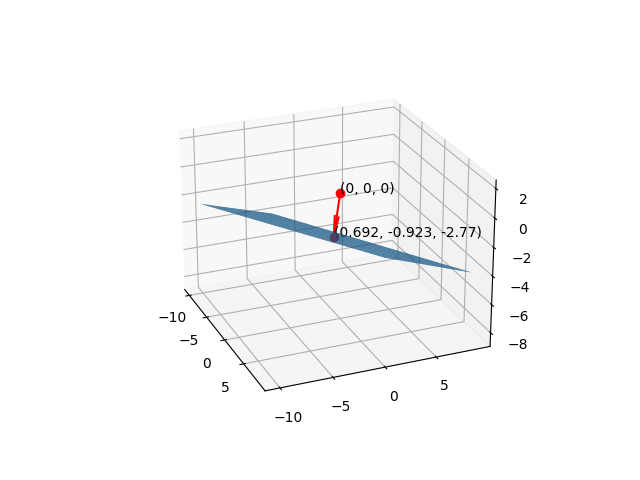
\includegraphics[width=\linewidth]{Graph_3D}
	\caption{Graph of the given plane}
\end{figure}

\end{document}  